\documentclass[8pt]{extarticle}

% Packages
\usepackage[T1]{fontenc}
\usepackage[utf8]{inputenc}
\usepackage{geometry}
\usepackage[colorlinks=true, urlcolor=blue, pdfborder={0 0 0}]{hyperref}
\usepackage{multicol} 
\usepackage{xcolor}
\usepackage{listings} %for SQL snippets
\usepackage{pdflscape} % for landscape pages
\usepackage{enumitem} %for formatting of lists
\usepackage{graphicx} %for scaling tabular environments
\usepackage{tabularx} %for allowing wrapping columns whilst respecting rescaling.
\usepackage{tcolorbox} %for highlighted boxes
\usepackage{amsmath}

\usepackage{lipsum} %for sample paragraphs, delete at end

%correct handling of _ inside inline code snippet
\lstset{
    language=Python,
    basicstyle=\ttfamily,
    literate={_}{{\_}}1
}


% Page configuration
\geometry{a4paper, landscape, top=10mm, bottom=10mm, left=10mm, right=10mm, columnsep=10mm,}

% no indent globally
\setlength{\parindent}{0pt}

% Python snippet environment
\lstdefinestyle{python}{
    language=Python,
    basicstyle=\small\ttfamily,
    keywordstyle=\color{blue},
    commentstyle=\color{gray},
    stringstyle=\color{teal},
    identifierstyle=\color{black},
    numberstyle=\tiny\color{gray},
    keywordstyle=[2]\color{purple},
    keywordstyle=[3]\color{orange},
    breaklines=true,
    showstringspaces=false,
    tabsize=4,
    %numbers=left,
    numbersep=5pt
}

% Lined separator for headings
\newcommand{\heading}[1]{%
    \noindent
    \rule{\linewidth}{0.4pt}
    \begin{center}
        \vspace{-1ex}
        \textbf{#1}        
        \vspace{-2.5ex}
    \end{center}
    \rule{\linewidth}{0.4pt}
}

\pagenumbering{gobble}

\begin{document}

% Remove page numbers for this page
\thispagestyle{empty} 

% Title
\begin{center}   
{\huge\textbf{EXCEL AND POWERQUERY CHEAT SHEET}}\\
\vspace*{0.5cm}
{\huge\textbf{Excel}}
\vspace*{0.75cm}
\end{center}

\begin{multicols}{3}
\setlength{\columnseprule}{1pt} % Add vertical line between columns


\heading{DUMMY DATA}

Some concepts will be best explained via an example, in which case, the following dummy data will be used:

\begin{center}
    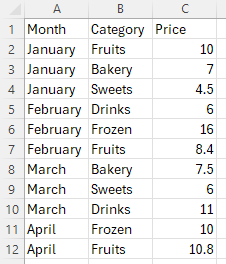
\includegraphics[width = 0.55\columnwidth]{images/dummy_data.png}
\end{center}

It shows purchases of foods by category over a range of months.

\heading{A SMALL NOTE ON DEFAULT CELL ALIGNMENT}

Strings are left-aligned by default. 

Numeric types and Dates are right-aligned by default.

\heading{RELATIVE V.S. ABSOLUTE REFERENCING}

Formulas (obtained by starting cell entry with "=") can reference other cells, either relatively or absolutely:
\begin{itemize}
\item Relative : Refers to a cell relative to the current position, adjusting as the formula is moved. Think: I want to reference the cell "X cells across and Y cells up."
\item Absolute: refers to a fixed cell that doesn’t change when the formula is moved, using dollar signs (\$). For example, \$A\$1 always refers to cell A1.
\end{itemize}

\begin{tcolorbox}[width=\columnwidth, colback=white!95!black]
Note: You can lock only the row or column by placing the dollar sign (\$) before only one of them e.g., \$A1 or A\$1.
\end{tcolorbox}

\columnbreak
\heading{BASIC FORMULAS/FUNCTIONS}


\begin{center}
    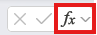
\includegraphics{images/insert_function.png}
    
    The insert function button
\end{center}

Functions can be added by typing "= ..." or pressing the Insert Function button and selecting a function. The Insert Function button also acts as a function helper when pressed whilst the cursor is inside the function argument brackets. 

Functions may also be found by navigating in the ribbon:

\[    \textbf{Formulas} \rightarrow \textbf{Function Library}\]

\begin{center}
    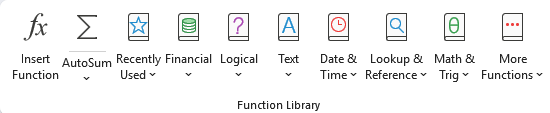
\includegraphics[width=\columnwidth]{images/function_library.png}
\end{center}

Formulas may be evaluated step-by-step (to assist with debugging, for example) via the use of 

\[    \textbf{Formulas} \rightarrow \textbf{Formula Auditing} \rightarrow \textbf{Evaluate Formula}\]

\heading{FORMATTING}

\begin{itemize}
    \item To format a cell as a number, navigate to 
    \[\textbf{Home} \rightarrow \textbf{Number}\]
        \begin{center}
        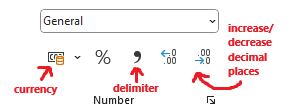
\includegraphics[width=0.6\columnwidth]{images/number.png}    
        \end{center}
    \item Use the format painter ($\textbf{Home} \rightarrow \textbf{Clipboard} \rightarrow \textbf{Format Painter}$) to paint the format of the current cell onto other cells. Click once to apply once, double-click to keep active.
    \item Cell styles can be used/created (i.e. background colour, text colour, number format) via $\textbf{Home} \rightarrow \textbf{Styles} \rightarrow \textbf{Cell Styles...}$. Modifying a style will automatically change all cells with that style applied.
    \item Conditionally formatting (accessed via $\textbf{Home} \rightarrow \textbf{Styles} \rightarrow \textbf{Conditional Formatting}$) applies formatting based on conditionals. 
    These can be edited via \newline    
    $\dots \rightarrow \textbf{Conditional Formatting} \rightarrow \textbf{Manage Rules}$
\end{itemize}

\heading{BASIC CHARTS}

Charts may be found in the ribbon via:

\[ \textbf{Insert} \rightarrow \textbf{Charts} \]

\begin{itemize}
    \item Highlight cells/select a table and choose a chart
    \item When selecting a chart, the Chart Design and Format tabs appear. 
    \item Chart Design allows selection of chart style, change the data selected, change chart type etc.
    \item Format allows fonts to be changed, as well as the addition of shapes etc.
    \item Also when selecting a chart, icons allowing the addition of Chart Elements, the changing of Chart styles, and application of Chart Filters (e.g. filter some rows/columns of data out) appear.    
        \begin{center}
        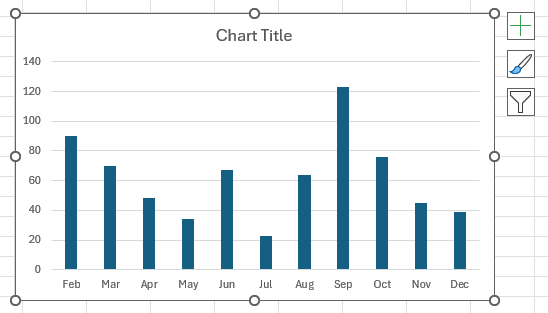
\includegraphics[width=0.9\columnwidth]{images/chart_example.png}    
        \end{center}
\end{itemize}

\columnbreak
\heading{EXCEL LISTS (SORTING AND FILTERING)}

These are single columns of related data (e.g. a list of names). Excel will automatically look for headers in the first row. This is useful for sorting and filtering.

\[\underline{\text{Sorting}}\]

\begin{itemize}
    \item To sort column(s): 
    \item Click into the column/highlight columns/click into table
    \item Navigate to \( \textbf{Data} \rightarrow \textbf{Sort \& Filter} \)
    \item To sort A-Z or Z-A, select the icon
    \item For more complicated sorts (e.g. sorting abbreviated months chronologically, click $\textbf{Sort}$ and Order by Custom List...
    \item Can add multiple (levels of) sorts, they will be carried out from top downwards.
\end{itemize}

\[\underline{\text{Filtering}}\]

\begin{itemize}
    \item To filter data in column(s): 
    \item Click into the column/highlight columns/click into table
    \item Navigate to \( \textbf{Data} \rightarrow \textbf{Sort \& Filter} \rightarrow \textbf{Filter}\)
    \item Dropdowns will appear in the cells of the column header(s)
    \item Filters can be cleared via \( \textbf{Data} \rightarrow \textbf{Sort \& Filter} \rightarrow \textbf{Clear}\)
\end{itemize}

\heading{SUBTOTAL}

Used to answer questions like "What were the total sale amounts for each item?" or "How much did I spend in each month?"

\begin{itemize}
    \item Sort the column we wish to take subtotals with respect to (this is because subtotals works by detecting changes in values in this column).
    \item highlight or click into list/range somewhere. Note that subtotal cannot be used with tables.
    \item $ \textbf{Data} \rightarrow \textbf{Outline} \rightarrow \textbf{Subtotal}$ gives the window in figure below (left).
    \item The "Use function:" dropdown lets you choose an aggregate function to use e.g. sum, average, mean...
    \item The "Add subtotal to:" box lets you select which column to apply subtotals to. In our dummy data, summing price is a good choice. (see figure, the left hand image)
    \item The result of "Ok" can be seen in the figure below (on the right). 
    \item Note: The 1,2,3, +, and - buttons can be used to expand, and condense groupings to various levels. 
\end{itemize}      
    \begin{center}
    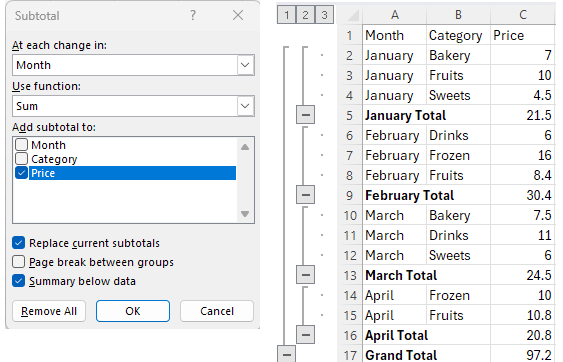
\includegraphics[width = 0.95\columnwidth]{images/subtotal.png}
    \end{center}

\heading{FORMAT AS TABLE}

Explicitly formatting as a table (as opposed to just having the data as a collection of columns) has many benefits, including
\begin{itemize}
    \item Allows addition of counts which respect filtering
    \item Allows, for example, alternating colouring of rows, which doesn't get destroyed by sorting, which improves readability
\end{itemize}
To achieve it, click into the "table" and navigate to 
\[ \textbf{Home} \rightarrow \textbf{Styles} \rightarrow \textbf{Format as Table}\]
Note that a Table Design tab has appeared.

\heading{REMOVING DUPLICATES}

To remove duplicates from a table:
\[ \textbf{Table Design} \rightarrow \textbf{Tools} \rightarrow \textbf{Remove Duplicates}\]

To remove duplicates from lists of data (i.e. data which is not formatted as a table):
\[ \textbf{Data} \rightarrow \textbf{Data Tools} \rightarrow \textbf{Remove Duplicates} \]

\columnbreak
\heading{DATABASE FUNCTIONS (DSUM, DCOUNT,...)}

These functions apply a function to a specified field/column that match given conditions/criteria. A list of such functions is: 

\begin{itemize}
    \item DSUM
    \item DCOUNT
    \item DAVERAGE
    \item DMIN, DMAX
    \item More can be found by clicking $\textbf{Insert Function}$ and querying for "database".
\end{itemize}

All such functions require the following arguments:

\begin{itemize}
    \item Database, Field, Criteria
    \item Database: This is the range of cells that make up the data
    \item Field: Label of the column the function should be applied to
    \item Criteria: A "mini-table" containing column headers and conditions that entries must satisfy to be included in the main function
\end{itemize}

Here is an example of applying some database functions to the dummy data. Notice that E2:F3 is a "mini-table", created to house the criteria:

\begin{center}
    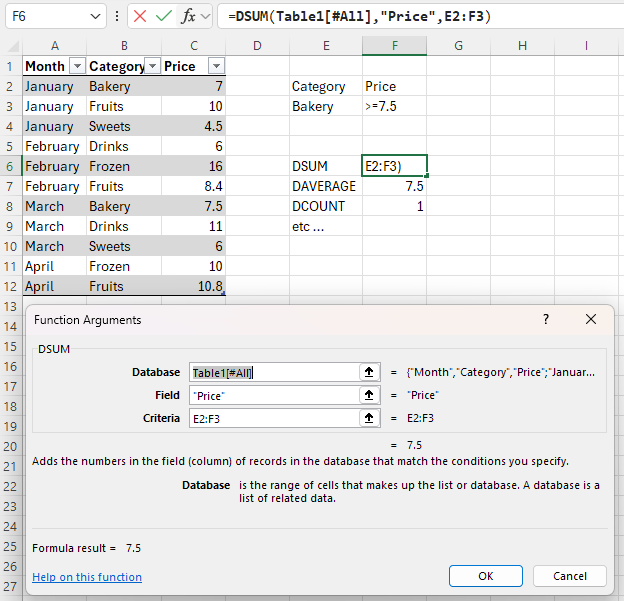
\includegraphics[width=0.98\columnwidth]{images/DFunctions.png}
\end{center}

\heading{DATA VALIDATION}

Data Validation allows us to set rules that entries to a cell must adhere to. It can be obtained by navigating to:
\[ \textbf{Data} \rightarrow \textbf{Data Tools} \rightarrow \textbf{Data Validation} \]

For example, the following would only allow values from the list $[A,B,C]$ to be inputted into the cells. You can also change the cell input message and error message.

\begin{center}
    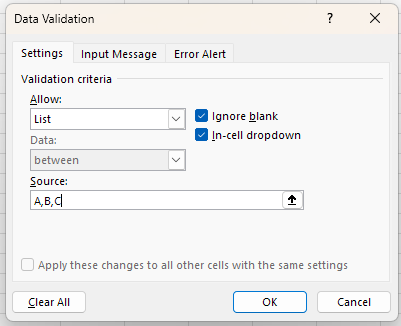
\includegraphics[width = 0.7\columnwidth]{images/DataValidation.png}
\end{center}

\heading{IMPORTING/EXPORTING DATA}

Data can be imported by navigating to

\[ \textbf{Data} \rightarrow \textbf{Get and Transform Data} \rightarrow \textbf{Get Data} \]

You can import data from many places, for example,

\begin{itemize}
    \item Files e.g. csv, json, pdfs
    \item Databases e.g. Microsoft Access, MySQL
    \item Other Sources e.g. Table/Range 
\end{itemize}

Importing data opens a window where there is a choice to Load, Load To, or Transform Data. 

\begin{itemize}
    \item Load - Load the data to a new worksheet
    \item Load To - allows loading to a specified location/worksheet. You can also load to a PivotTable report immediately.
    \item Transform Data - opens the data in PowerQuery.
\end{itemize}

To export data, navigate to 

\[\textbf{File} \rightarrow \textbf{Save As} \]

and choose the required file type from the dropdown.

\columnbreak
\heading{PIVOT TABLES}

Pivot Tables create aggregated values by grouping data from an original table. They are similar to applying an aggregate function, like SUM or COUNT, to data grouped by two or more columns. The key difference is that these field labels, used to define the groupings, appear on the rows and columns, creating a grid-like structure.

To use: 

\begin{itemize}
    \item Tip: It is better to format the range of data as a table.
    \item Navigate to $\textbf{Insert} \rightarrow \textbf{Tables} \rightarrow \textbf{PivotTable}$ - select range of cells/table and the desired location of the pivot table.
    \item Using the new window on the right (see below image), drag column headers/field's into Filters/Columns/Rows/Values boxes to use them in the pivot table.
    \begin{center}
        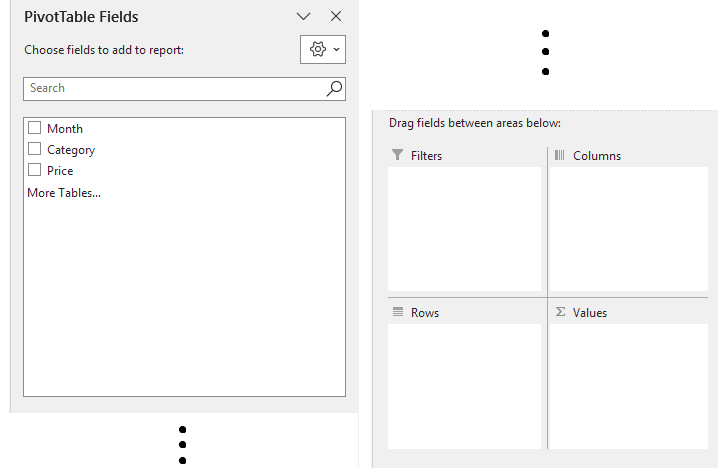
\includegraphics[width=0.95\columnwidth]{images/pivottable-menu.png}
    \end{center}
    \item Filters will use the data in the field's column as a filter. Row/Column uses the data in the field's column to group the data. Values uses the values in the field's column to aggregate (usually this is numeric).
    \item The "Value Field Settings" option for fields in the Values box allows the aggregate function to be chosen e.g. SUM, COUNT, AVERAGE etc.
\end{itemize}

\columnbreak
For example, a pivotable for the dummy data, where data is grouped by Month on columns, and Category on rows, with aggregate data being max price:
\begin{center}
        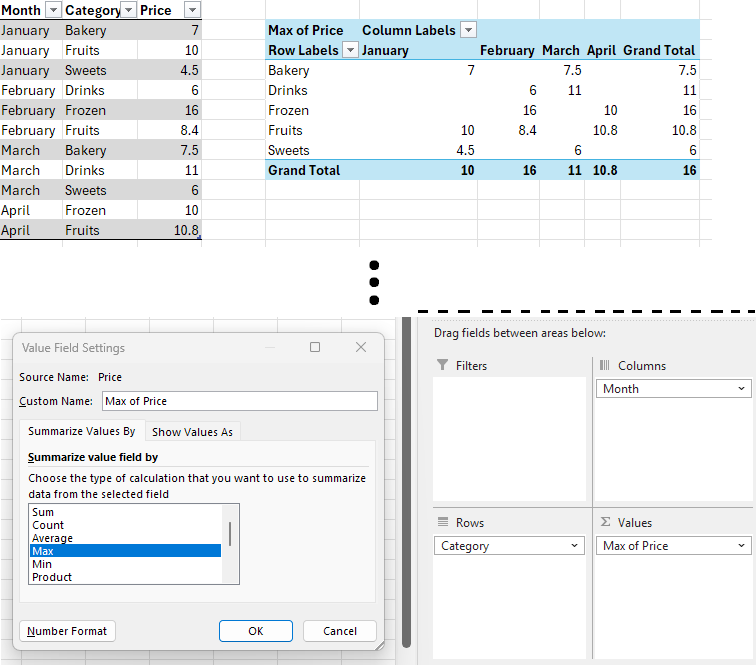
\includegraphics[width=0.9\columnwidth]{images/pivottable-example.png}
    \end{center}

\begin{center}
    \underline{Grouping rows/columns within pivot tables}
\end{center}

\begin{itemize}
    \item Highlight columns/rows you want to group
    \item $\textbf{PivotTable Analyse} \rightarrow \textbf{Group} \rightarrow \textbf{Group Selection}$
\end{itemize}

\begin{center}
    \underline{Formatting pivot tables}
\end{center}

\begin{itemize}
    \item Warning: $\textbf{Home} \rightarrow \textbf{Number}$ formats the cells, not the table itself. If pivot table change size, all the cells may not have the formatting applied
    \item Instead use Value Field Settings $\rightarrow$ Number Format from within the Values box of the pivot table window.
\end{itemize}

\begin{center}
    \underline{Other aggregate functions e.g. lead/lag}
\end{center}

\begin{itemize}
    \item To obtain functions such as lead/lag/running total and more:
    \item Go to Value Field Settings $\rightarrow$ Show Values As and choose suitable options.
\end{itemize}

\begin{center}
    \underline{Drill down}
\end{center}

Double-clicking a pivot table value produces a new table in a new worksheet displaying all data making up that value.

\columnbreak
\begin{center}
    \underline{Charts}
\end{center}

\begin{itemize}
    \item To create charts using pivot table data:
    \item $\textbf{PivotTable Analyse} \rightarrow \textbf{Tools} \rightarrow \textbf{PivotChart}$
\end{itemize}

\begin{center}
    \underline{Filtering pivot tables}
\end{center}

\begin{itemize}
    \item Drag column header/field into the Filter box within the pivot table window. 
    \item Use the dropdown menu that is now present in the pivot table to filter the data
\end{itemize}

Alternatively, a more interactive way to filter can be done using 

\[\textbf{PivotTable Analyse} \rightarrow \textbf{Filter} \rightarrow \textbf{Insert Slicer}\]

After selecting the column headers/fields you want to filter with respect to, an interactive window will appear, allowing you to filter items. This is ideal for dashboards.

\heading{POWER PIVOT}

Power Pivot allows the creation of pivot tables using data from multiple tables that may be related in some way (this involves methods similar to that of an SQL Join).

\begin{itemize}
    \item Need a data model to connect the tables
    \item To add tables to a Data Model, click into them and navigate to $\textbf{PowerPivot} \rightarrow \textbf{Tables} \rightarrow \textbf{Add to Data Model}$
    \item This opens a new window (PowerPivot for Excel) containing the table data
    \item Repeat this for all relevant tables.
    \item The tables are now present on different sheets within PowerPivot for Excel
\end{itemize}

For the rest of this section, all navigations occur in PowerPivot for Excel. We also need another table to link to our dummy data. For this we use the following, showing costs to source items for each month (the idea being that profit will be Price - Source Cost):
\begin{center}
    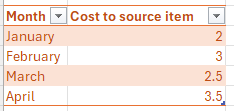
\includegraphics[width=0.6\columnwidth]{images/dummy2.png}
\end{center}

\begin{center}
    \underline{Creating relationships between tables}
\end{center}
To create relationships/links between columns in different tables:
\begin{itemize}
    \item $\textbf{Home} \rightarrow \textbf{Diagram View}$
    \item Drag \& drop column/field names to create a link (drag from the parent to the child)
\end{itemize}
Alternatively,
\begin{itemize}
    \item $\textbf{Home} \rightarrow \textbf{Data View}$
    \item Right click on the parent column header and select "Create Relationship"
    \item Select the table the desired child column belongs to from the dropdown menu and click the child column header.
\end{itemize}

\begin{center}
    \underline{PivotTable with linked tables}
\end{center}

We can use pivottables using data from the linked tables together.

\begin{itemize}
    \item $\textbf{Home} \rightarrow \textbf{PivotTable}$
    \item This will return to Excel, choose where to place the table
    \item Now column headers/fields from all linked tables are available to use within the pivot table - they are able to "see each other" through the links between the tables.
\end{itemize}

\begin{center}
    \underline{PowerPivot KPI}
\end{center}

Note: KPI stands for key performance indicator.

\begin{itemize}
    \item Add an aggregate function to a column within PowerPivot (e.g. AVERAGE) using $\textbf{Home} \rightarrow \textbf{Calculations} \rightarrow \textbf{AutoSum (dropdown)}$.
    \item This is the value the indicator will be based on (e.g. is some value much lower, about equal or much greater than the average)
    \item Add KPI via $\textbf{Home} \rightarrow \textbf{Calculations} \rightarrow \textbf{Create KPI}$
    \item Add a target value and define thresholds (where red becomes yellow becomes green).
    \item To edit a KPI, right-click the cell with the aggregate function and select "Edit KPI settings"
    \item These KPI indicators are available and can be used in pivot tables.
\end{itemize}

\heading{TIPS FOR WORKING WITH LARGE DATA SETS}

\begin{center}
    \underline{Freeze rows/columns}
\end{center}

\begin{itemize}
    \item $\textbf{View} \rightarrow \textbf{Window} \rightarrow \textbf{Freeze Panes}$
    \item This freezes all cells which are to the left or above the currently selected cell.
\end{itemize}
\columnbreak
\begin{center}
    \underline{Create column/row grouping}
\end{center}

\begin{itemize}
    \item Select row/column headers/indices you want to group 
    \item $\textbf{Data} \rightarrow \textbf{Outline} \rightarrow\textbf{Group}$
\end{itemize}

\begin{center}
    \underline{Linking worksheets}
\end{center}

\begin{itemize}
    \item We can create formulas using cells from other sheets by referring them in the following way.
    \item \{other\_sheet\_name\}!\{cell\_number\}. For example, importing cell A1 from a sheet called "SupplyCostsSheet" is done via SupplyCostsSheet!A1
\end{itemize}

\begin{center}
    \underline{Consolidating data}
\end{center}

\begin{itemize}
    \item To consolidate data from different tables (including when the tables are in different sheets you can do the following:
    \item $\textbf{Data} \rightarrow \textbf{Data Tools} \rightarrow \textbf{Consolidate}$
    \item Choose function (i.e. what function will you use to combine data from the different sources. e.g. if you want a grant total for sales for each item, use SUM)
    \item Add all tables as references by highlighting them/adding their table name to the "Reference" box and pressing "Add"
    \item Select whether you want to use column header labels/ row index labels (or both) from the source data.
\end{itemize}

\heading{CONDITIONAL FUNCTIONS/FORMATTING}

\begin{center}
    \underline{Excel name ranges}
\end{center}

You can name a range of cells for later reference, this is some sort of middle ground between having a range of cells and having a table. 

\begin{itemize}
    \item Select cell range
    \item Rename in the name box (to the bottom left of the ribbon).
    \item Can use this name to reference this range of cells. Note that it is an absolute reference.
    \item Use the dropdown in the name box to select and navigate to named cell ranges
    \item To manage names: 
    
    $\textbf{Formulas} \rightarrow \textbf{Defined Names} \rightarrow \textbf{Name Manager}$.
\end{itemize}

\columnbreak
\begin{center}
    \underline{Conditional functions}
\end{center}

\begin{itemize}
    \item IF
    \begin{itemize}
        \item Arguments:
        \begin{itemize}
            \item Logical\_test - a value or expression that can be evaluated to TRUE or FALSE
            \item Value\_if\_true - the value returned if the test is TRUE
            \item Value\_if\_false - the value returned if the test is FALSE
        \end{itemize}
    \item Example: 
    
    =IF(A1>1,"Greater than 1", "Not greater than 1")
    \end{itemize}
\end{itemize}

\begin{itemize}
    \item AND
    \begin{itemize}
        \item Arguments:
        \begin{itemize}
            \item Logical1 - a value or expression that can be evaluated to TRUE or FALSE
            \item Logical2 - another value or expression that can be evaluated to TRUE or FALSE
            \item Logical3 - ...
            \item (You can add up to 255 logical expressions)
        \end{itemize}
        \item Return:

        Returns TRUE if all logical expressions evaluate to TRUE, otherwise, it returns FALSE
    \end{itemize}
\end{itemize}

\begin{itemize}
    \item COUNTIF
    \begin{itemize}
        \item Arguments:
        \begin{itemize}
            \item Range - the range of cells from which you wish to count blank cells
            \item Criteria - logical criteria the cell has to meet in order to be counted
        \end{itemize}
        \item Return:

        Returns the number of cells in the range that meet the given criteria
        \item Example:

        =COUNTIF(A1:A5, ">5")
    \end{itemize}
\end{itemize}

\begin{itemize}
    \item SUMIF - performs similarly to COUNTIF, but can use different ranges for the cells which have to satisfy criteria, and the cells which will actually be summed up. 
    \begin{itemize}
    \item Example: 

    Using dummy data, to sum total price of Bakery items we would do: =SUMIF(B2:B12, "Bakery", C2:C12)
    \end{itemize}
\end{itemize}

\begin{itemize}
    \item IFERROR
    \begin{itemize}
        \item Arguments:
        \begin{itemize}
            \item Value - an expression or value (which may cause an error)
            \item Value\_if\_error - the value the function will return if there is an error with the "Value" argument.
        \end{itemize}
        \item Return:

        Returns Value if there's no error, and Value\_if\_error if there is an error.
        \item Example:

        =IFERROR(5/0,"Bad: Dividing by zero")
    \end{itemize}
\end{itemize}

\heading{LOOKUP FUNCTIONS}

\begin{itemize}
    \item VLOOKUP
    
    Looks for the first match to a value in the first column of a range of cells, and returns the value in the column specified. By default, the first column should be sorted in ascending order.
    \begin{itemize}
        \item Arguments:
        \begin{itemize}
            \item Lookup\_value - the value you wish to search for from the first column
            \item Table\_array - the range of cells or table name
            \item Col\_index\_num - the column number from the range of cells passed. Note that the first column is indexed 1.
            \item Range\_lookup - TRUE if you are happy with the closest match (for this, the column should be sorted). FALSE if you want an exact match (this can return N/A if no match is found).
        \end{itemize}
    \end{itemize}
\end{itemize}

\begin{itemize}
    \item HLOOKUP 
    
    Looks for the first match to a value in the first row of a range of cells, and returns the value in the row specified. The first row is indexed by 1. 
    
    This works the same as VLOOKUP, including the same arguments, but with the roles of columns and rows swapped.
\end{itemize}

\begin{itemize}
    \item INDEX 
    
    Returns the value within the cell at a given row and column number. (Both row and column numbering starts at 1).
    \begin{itemize}
        \item Arguments:
        \begin{itemize}
            \item Array 
            \item Row\_num - the row from which to return the value
            \item Col\_num - the column from which to return the value
        \end{itemize}
    \end{itemize}
\end{itemize}

\columnbreak
\begin{itemize}
    \item MATCH 
    
    Returns the relative position of an item in a row or column that matches a specified value.
    \begin{itemize}
        \item Arguments:
        \begin{itemize}
            \item Lookup\_value
            \item Lookup\_array - must be a single row or column.
            \item Match\_type - one of -1,0,1. (if using $\pm 1$, ensure the data is sorted.)
            
            0 = exact match, 
            
            -1 = smallest value greater than or equal to the lookup value, 
            
            1 = greatest value smaller than or equal to the lookup value.
        \end{itemize}
    \end{itemize}
\end{itemize}

\heading{TEXT FUNCIONS}

\begin{itemize}
    \item LEFT/RIGHT
    
    Returns the specified number of characters from the start/end of a string
    \begin{itemize}
        \item Arguments:
        \begin{itemize}
            \item Text
            \item Num\_chars - the number of characters to return.
        \end{itemize}
    \end{itemize}
\end{itemize}

\begin{itemize}
    \item MID
    
    Returns the specified number of characters from the middle of a string, at a choosen start point
    \begin{itemize}
        \item Arguments:
        \begin{itemize}
            \item Text
            \item Start\_num - the index of the first character you want to extract
            \item Num\_chars - the number of characters to return.
        \end{itemize}
    \end{itemize}
\end{itemize}

\begin{itemize}
    \item LEN
    
    Returns the length of the text
    \begin{itemize}
        \item Arguments:
        \begin{itemize}
            \item Text
        \end{itemize}
    \end{itemize}
\end{itemize}

\begin{itemize}
    \item SEARCH
    
    Returns the character index at which the first occurrence of the target string is found
    \begin{itemize}
        \item Arguments:
        \begin{itemize}
            \item Find\_text - the text you want to find
            \item Within\_text - the text you want to search in.
        \end{itemize}
    \end{itemize}
\end{itemize}

\columnbreak
\begin{itemize}
    \item CONCATENATE
    
    Joins several strings into a single string
    \begin{itemize}
        \item Arguments:
        \begin{itemize}
            \item Text1 
            \item Text2
            \item (Can have up to 255 arguments, up to Text255)
        \end{itemize}
    \end{itemize}
\end{itemize}

\heading{"NEW" EXCEL FUNCTIONS (POST 2019)}

\begin{itemize}
    \item FILTER
    
    Filter a range or array
    \begin{itemize}
        \item Arguments:
        \begin{itemize}
            \item Array
            \item Filter - an array of booleans where TRUE denotes a row or column to keep. This can be obtained via a logical condition 
            
            e.g. 'my\_table[my\_column] = "some value" '.
        \end{itemize}
    \end{itemize}
\end{itemize}

\begin{itemize}
    \item SORT
    
    Sort an array 
    \begin{itemize}
        \item Arguments:
        \begin{itemize}
            \item Array
            \item Sort\_index - the index of the column/row you want to sort with respect to 
            \item Sort\_order - +1 for ascending, -1 for descending]
            \item By\_col - TRUE to sort the columns, FALSE to sort the rows (default)
        \end{itemize}
    \end{itemize}
\end{itemize}

\begin{itemize}
    \item UNIQUE
    
    Returns the unique values from an array/list
    \begin{itemize}
        \item Arguments:
        \begin{itemize}
            \item Array
            \item By\_col - TRUE for return unique rows, FALSE for return unique columns
            \item Exactly\_once - TRUE for returning rows/columns that appear exactly once, FALSE for returning all unique rows/columns, even if they appear multiple times (default)
        \end{itemize}
    \end{itemize}
\end{itemize}

\columnbreak
\begin{itemize}
    \item XLOOKUP
    
    Looks for a value in a lookup range, and returns a corresponding value from a return range.
    \begin{itemize}
        \item Arguments:
        \begin{itemize}
            \item Lookup\_value
            \item Lookup\_array - the range to search for the lookup value
            \item Return\_array - the range from which to return the value.
            \item If\_not\_found - what do return if no match is found
            \item Match\_mode - specify the match type:
            
            0 - Exact match. If none found, return \#N/A. This is the default.
            
            -1 - Exact match. If none found, return the next smaller item.
            
            1 - Exact match. If none found, return the next larger item.
        \end{itemize}
    \end{itemize}
\end{itemize}

\begin{itemize}
    \item SWITCH
    
    Essentially a multi-if statement, i.e. if ValueN then return ResultN
    \begin{itemize}
        \item Arguments:
        \begin{itemize}
            \item Expression - the value/expression to be evaluated
            \item Value1 - value to be compared to expression
            \item Result1 - returned if expression matches Value1
            \item (Value2, Result2, etc)
        \end{itemize}
    \end{itemize}
\end{itemize}

\begin{itemize}
    \item TEXTJOIN
    
    Essentially concatenate, but more streamlined if a custom delimiter is used
    \begin{itemize}
        \item Arguments:
        \begin{itemize}
            \item Delimiter
            \item Ignore\_empty - if TRUE it ignores empty cells if a range is passed
            \item Text1 - text or range to be joined
            \item (Text2, ..., Text252)
        \end{itemize}
    \end{itemize}
\end{itemize}

\begin{itemize}
    \item TEXTSPLIT
    
    Splits text into rows or columns
    \begin{itemize}
        \item Arguments:
        \begin{itemize}
            \item Text - the text to split
            \item Col\_delimiter - character ot string to split columns by
            \item Row\_delimiter - character ot string to split rows by
            \item There are also ignore\_empty and match\_mode arguments.
        \end{itemize}
    \end{itemize}
\end{itemize}

\heading{AUDITING}

\begin{center}
    \underline{Tracing precedents/dependents}
\end{center}

We can see which cells affect a current calculation, or vice versa using auditing. This is known as tracing precedents/dependents. This is done as follows:
\begin{center}
$\textbf{Formulas} \rightarrow \textbf{Formula Auditing} $

$\rightarrow \textbf{Trace Precedents/Trace Dependents}$
\end{center}

\begin{center}
    \underline{Watch window}
\end{center}

This is somewhat reminiscent of having sheets in different windows with split screen. The watch window does what it says, it allows you to watch cells as you interact with the workbook. This is done via
\[\textbf{Formulas} \rightarrow \textbf{Formula Auditing} \rightarrow \textbf{Watch Window}\]

\begin{center}
    \underline{Show formulas}
\end{center}

Shows formulas in the cells, rather than the final value. This is handy for debugging etc.
\[\textbf{Formulas} \rightarrow \textbf{Formula Auditing} \rightarrow \textbf{Show Formulas}\]

\heading{PROTECTING WORKSHEETS AND BOOKS}

\begin{itemize}
    \item Protecting cells:

    All cells have a lock (which is enabled by default). This is merely the ability to be locked. Before protecting a cell, disable the lock on any cells you want to keep free to edit. This is done via highlighting the cell(s), pressing Ctrl+Shift+F (format window), going to the protection tab, and unchecking Locked. 

    To protect the sheet, go to 

    \[\textbf{Review} \rightarrow \textbf{Protect} \rightarrow \textbf{Protect Sheet}\]

    to unprotect, go to 
    
    \[\textbf{Review} \rightarrow \textbf{Protect} \rightarrow \textbf{Unprotect Sheet}\]

    \item Protect workbook structure:

    This ensures you cannot add/remove/change sheets themselves

    \[\textbf{Review} \rightarrow \textbf{Protect} \rightarrow \textbf{Protect Workbook}\]

    \item Adding password to a workbook

    \[ \textbf{File} \rightarrow \textbf{Info} \rightarrow \textbf{Protect Workbook}\]
    \[ \rightarrow \textbf{Encrypt with Password}\]
    To remove password, re-encrypt with a blank password field.
\end{itemize}

\columnbreak
\heading{WHAT IF ANALYSIS}

What-if analysis allows you to try out different inputs (scenarios) for formulas.

\[ \textbf{Data} \rightarrow \textbf{Forcast} \rightarrow \textbf{What if analysis}\]

\begin{itemize}
    \item Goal Seek: Determines what value needs to be inserted into an input cell to achieve the desired value in the output cell. 

    Arguments
    \begin{itemize}
        \item Set cell: the output cell, whose value you wish to control
        \item To value: the value you want the output cell to achieve
        \item By changing cell: the input cell whose values you allow to change
    \end{itemize}

    \item Data Tables: A table designed to neatly arrange and calculate formulas on a range of changing arguments. 

    They work as follows. Suppose we have a formula with inputs B1 and B2, producing an output in B3. For example:
    \begin{center}
        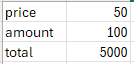
\includegraphics[width=0.3\columnwidth]{images/small_formula_eg.png}
    \end{center}
    We then create a grid, with different values of price as column headers, and different values for amount as row indices. We make a reference to the formula output in the top-left of the newly-created grid.    
    \begin{center}
        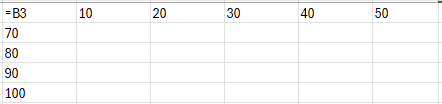
\includegraphics[width=0.9\columnwidth]{images/empty_grid.png}
    \end{center}
    Highlight the whole grid (including the headers and indices) and navigate to $\textbf{Data Table}$. Add cell B1 (the cell containing the price) as the row input cell, then add cell B2 (the cell containing the amount) as the column input cell. Press OK. This gives the following completed grid.     
    \begin{center}
        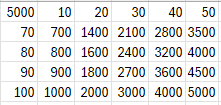
\includegraphics[width=0.6\columnwidth]{images/complete_data_table.png}
    \end{center}
    
    \item Scenario Manager: you can add scenarios which allow you to set multiple sets of values for the same set of cells and flick between them.
\end{itemize}

There is also a linear programming solver built into Excel 

\[ \textbf{Data} \rightarrow \textbf{Analyse} \rightarrow \textbf{Solver}\]

\heading{EXCEL MACROS}

You can record and reuse a recorded sequence of steps to automate task (such as formatting etc). All tools can be found in 

\[\textbf{Developer} \rightarrow \textbf{Code}\]

Macros can be recorded with $\textbf{Record Macro}$, they can be edited, renamed, deleted etc by pressing $\textbf{Macros}$. They can be customised further with Visual Basic.

To assign a button to a macro go to 

\[\textbf{Developer} \rightarrow \textbf{Controls} \rightarrow \textbf{Insert} \rightarrow \textbf{Button} \]

\heading{VISUAL BASIC}

to do...
\vspace*{\fill}
\end{multicols}

%EXCEL COURSE ENDED HERE. THE REST OF THE CHEAT SHEET COVERS POWERQUERY WHICH WAS IN IT'S OWN SEPARATE COURSE

\newpage
% Remove page numbers for this page
\thispagestyle{empty} 
\begin{center}   
{\huge\textbf{PowerQuery}}\\
\vspace*{0.75cm}
\end{center}

\begin{multicols}{3}
\setlength{\columnseprule}{1pt} % Add vertical line between columns

\heading{GETTING STARTED}

All PowerQuery related tools can be found at 
\[\textbf{Data} \rightarrow \textbf{Get \& Transform Data} \]

PowerQuery prefers to work with tables as opposed to ranges of cells.

PowerQuery may be opened via 
\[\textbf{Data} \rightarrow \textbf{Get \& Transform Data} \rightarrow \textbf{Get Data} \]
\[\rightarrow \textbf{Launch PowerQuery Editor}\]

This opens a blank window, methods to add data can be found in the $\textbf{Home}$ tab. However, there are better ways to get data into PowerQuery.

\heading{RETRIEVING DATA}

We can open data from various sources inside PowerQuery - we mention some of the them here, all paths begin with 
\[\textbf{Data} \rightarrow \textbf{Get \& Transform Data} \rightarrow \textbf{Get Data} \rightarrow \dots\]
\begin{itemize}
    \item  From Excel File:
    
    $\dots \rightarrow \textbf{From File} \rightarrow \textbf{Excel Workbook}$
    \begin{itemize}
        \item Select the workbook from file explorer
        \item A navigator window will appear, allowing you to choose which tables from the workbook to import
    \end{itemize}
    \item From Excel Table within current worksheet:
    
    $\dots \rightarrow \textbf{From Other Sources} \rightarrow \textbf{From Table/Range}$
    \item From Text File:

    $\dots \rightarrow \textbf{From File} \rightarrow \textbf{From Text/CSV}$
    \columnbreak
    \item From DataBase:

    $\dots \rightarrow \textbf{From Database} \rightarrow \dots$
    \begin{itemize}
        \item Can select which tables or queried tables you wish to import within the navigator window that pops up
    \end{itemize}
    \item From Folder:

    $\dots \rightarrow \textbf{From File} \rightarrow \textbf{From Folder}$
    \begin{itemize}
        \item This is useful if you wish to, for example, import and merge a collection of csv files which are in the same folder (say monthly data you wish to merge into yearly data)
    \end{itemize}
    \item From the web:

    $\dots \rightarrow \textbf{From Other Sources} \rightarrow \textbf{From Web}$
    \begin{itemize}
        \item Insert URL of the webpage
        \item All <table> elements will appear in the navigator, select the tables you wish to import.
    \end{itemize}
\end{itemize}

\heading{TRANSFORMING DATA}

\begin{center}
    \underline{Set/Remove column headers}
\end{center}

If the first row has not been registered as the table headers (or the first row has incorrectly been registered as headers), go to $\textbf{Transform} \rightarrow \textbf{Table} \rightarrow \textbf{Use First Row as Headers ...}$

\begin{center}
    \underline{Setting Data Types}
\end{center}

Click the column header and navigate to 
\[\textbf{Home} \rightarrow \textbf{Transform} \rightarrow \textbf{Data Type ...}\]
Alternatively, click the icon in the top left of the column header cell to change data type. 

\begin{center}
    \underline{Splitting Column Data into multiple columns}
\end{center}

Click the column header and navigate to 
\[\textbf{Home} \rightarrow \textbf{Transform} \rightarrow \textbf{Split Column}\]
For example, transforming the price column into a column for whole pounds and another for pence is achieved as follows:
\begin{center}
    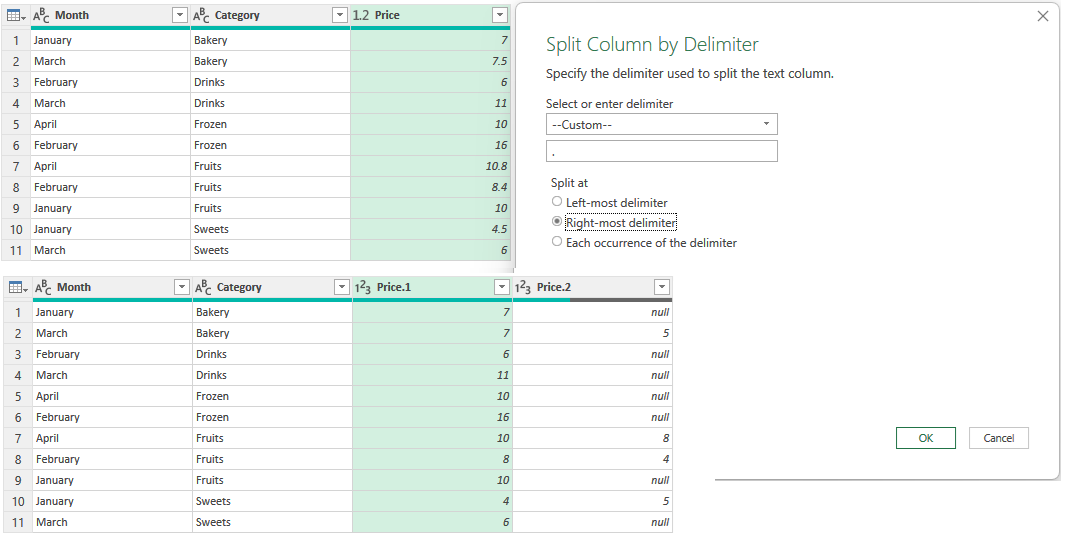
\includegraphics[width=\columnwidth]{images/split_column.png}
\end{center}

\begin{center}
    \underline{Formatting Text-based columns}
\end{center}
\[\textbf{Transform} \rightarrow \textbf{Text Column} \rightarrow \textbf{Format...}\]
Have options to set text to UPPERCASE, lowercase, Capitalised, Trim, Clean (removes all non-printable characters e.g. $\backslash$n).\\

Can also right-click whilst in a column and select "Replace Values", this allows the replacement of special characters by selecting "Advanced options" and "Replace using special characters".

\begin{center}
    \underline{Removing duplicate rows}
\end{center}
\[\textbf{Home} \rightarrow \textbf{Reduce Rows} \rightarrow \textbf{Remove Rows...}\]\[ \rightarrow \textbf{Remove Duplicates}\]

\begin{center}
    \underline{Filling columns}
\end{center}
Right Click column, "Fill" and then choose "Up" or "Down". This replaces null values in a column with the first non-null value found below/above it.

For example, fill down achieves the following:
\begin{center}
    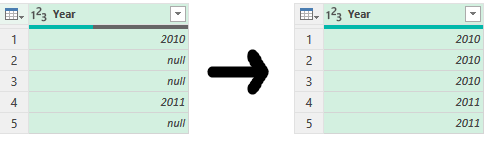
\includegraphics[width=0.9\columnwidth]{images/filldown.png}
\end{center}

\columnbreak
\heading{SORTING AND FILTERING}

\begin{center}
    \underline{Sorting}
\end{center}

On the column header, press the down arrow (on the right hand side of the cell) and select the sort you want. 

To apply a multi-level sort, sort the columns from highest priority to lowest priority - you will know a multi-sort is happening because the column headers will contain the numbers "1", "2", etc denoting the priority of the column in the multi-sort e.g. 
\begin{center}
    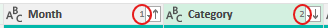
\includegraphics[width=\columnwidth]{images/multi-level-sort.png}
\end{center}

\begin{center}
    \underline{Filtering}
\end{center}

On the column header, press the down arrow (on the right hand side of the cell). Use the checkbox to manually filter, or use the "\{Data Type\} Filters" option to apply conditional filters (the filters available depend on the data type).

\heading{CLOSE AND LOAD OPTIONS}

\begin{itemize}
    \item Close \& Load - loads the table to a new worksheet in the Excel workbook.
    \item Close \& Load to - opens the following window
    \begin{center}
        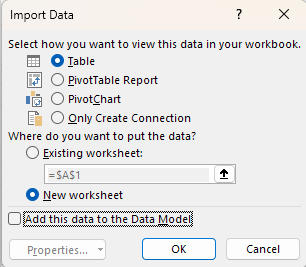
\includegraphics[width=0.6\columnwidth]{images/close_and_load_to.png}
    \end{center}
    \begin{itemize}
        \item Can open as a Table, PivotTable Report or Only Create Connection. The last option creates a connection which can be found in $\textbf{Data} \rightarrow \textbf{Queries and Connections}$ but won't load the table itself into the workbook.
    \end{itemize}
\end{itemize}
\columnbreak
\heading{PIVOT, UNPIVOT AND TRANSPOSING DATA}

\begin{center}
    \underline{Transposing data}
\end{center}

\[\textbf{Transform} \rightarrow \textbf{Table} \rightarrow \textbf{Transpose}\]

This turns rows of data into columns of data and vice versa.

\begin{center}
    \underline{Pivoting a column}
\end{center}

\begin{itemize}
    \item click into column you want to pivot
    \item $\textbf{Transform} \rightarrow \textbf{Any Column} \rightarrow \textbf{Pivot Column}$
    \item Choose another column as the values column 
    \item Use advanced options to choose the aggregate function to use.
\end{itemize}

For example, pivoting our dummy data by Category with the price column as the values column results in:
\begin{center}
    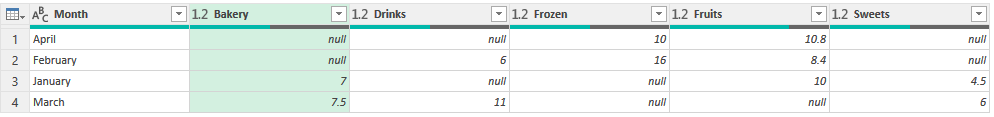
\includegraphics[width=0.98\columnwidth]{images/pivot_column.png}
\end{center}

\begin{center}
    \underline{Unpivoting columns}
\end{center}

This is the inverse of pivoting. Select multiple columns and unpivoting will replace them with two columns; one based on the column headers, and the other based on the values of the pivoted table.
\[\textbf{Transform} \rightarrow \textbf{Any Column} \rightarrow \textbf{Unpivot Columns...}\]\[ \rightarrow  \textbf{Unpivot Only Selected Columns} \]

\heading{GROUPING DATA}

\[\textbf{Home} \rightarrow \textbf{Transform} \rightarrow \textbf{Group By}\]

\begin{itemize}
    \item Basic: Select column as grouping column from the dropdown. On the next row give the new column a name, select an aggregate function, and select the column from which to take the values (for example, this could be a price/amount column).
    \item Advanced: Gives the option to group by multiple columns and/or use multiple aggregate functions on multiple value columns.
\end{itemize}

\columnbreak
\heading{ADDING COLUMNS}

There are many options for adding columns, which can be found at 
\[\textbf{Add Column} \rightarrow \dots\]
Some of these options include:
\begin{itemize}
    \item Column based on conditions (in $\textbf{General}$)
    \item An index column (in $\textbf{General}$)
    \item A duplicate/copy of an existing column  (in $\textbf{General}$)
    \item Columns based on data type (e.g. length of entries in cells of text based columns, or statistics based on numeric columns)
\end{itemize}

\heading{WORKING WITH MULTIPLE SOURCES}

In many cases, the data we want will be split over multiple sources. We can combine these using a merge (think SQL Join) or append (stacking them vertically, note column headers must match).

\begin{itemize}
    \item Merge
    \begin{itemize}
        \item Open two tables in PowerQuery that you want to merge.
        \item (Can open tables within PowerQuery via $\textbf{Home} \rightarrow \textbf{New Query} \rightarrow \textbf{New Source}$)
        \item To merge tables and create a new table:
        
        $\textbf{Home} \rightarrow \textbf{Combine} \rightarrow \textbf{Merge Queries ...} \rightarrow \textbf{Merge Queries As New}$
        \item Select the tables, the column to join on, and the join type (e.g. left, right, inner, etc)
    \end{itemize}
    \item Append
    \begin{itemize}
        \item This is used to stack tables on top of each other (think, combining monthly data into yearly data)
        \item The column headers in the two tables MUST match. 
        \item $\textbf{Home} \rightarrow \textbf{Combine} \rightarrow \textbf{Append Queries ...} \rightarrow \textbf{Append Queries As New}$
    \end{itemize}
\end{itemize}

\columnbreak
\heading{$M \times 1$ TABLE $\rightarrow m \times n$ TABLE METHOD}

Data presented in a single column i.e. stacked vertically (e.g. multiple people's name and age being stored vertically with the rows name, address, name, address, name, address, ...) is impossible to analyse. 

To fix this, we want to transform this data into 2 columns of name and address, with each entry being it's own row.

For example:
\begin{center}
    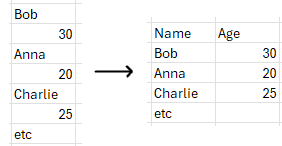
\includegraphics[width=0.65\columnwidth]{images/Mx1_to_mxn.png}
\end{center}

\begin{itemize}
    \item Add index column 
    
    ($\textbf{Add Column} \rightarrow \textbf{General} \rightarrow \textbf{Index Column}$)
    \item Add "modulo column" based on the index column. The modulo number will be the number of columns you want (e.g. for the above we would do modulo 2).
    
    ($\textbf{Add Column} \rightarrow \textbf{From Number} \rightarrow \textbf{Standard...} \rightarrow \textbf{Modulo}$)
    \item Add "integer division" column. Again, divide by the number of columns you want.
    
    ($\textbf{Add Column} \rightarrow \textbf{From Number} \rightarrow \textbf{Standard...} \rightarrow \textbf{Divide (Integer)}$)
    \item The Integer-Division column gives the row number for the new layout, and the modulo column gives the column number.
    \item Pivot using the modulo column (the values column should be chosen to be the column containing the original data).
    \item Group by the Integer-Division column, press "advanced" in the group-by window and then create a relevant name and select "max" as the aggregate function for each of the columns with data (this will choose the non-null value).
    \item Delete the Integer-Division column
\end{itemize}

\heading{PARAMETERS}

Replace hard-coded/static filter values with a variable one a.k.a. a parameter.

\[\textbf{Home} \rightarrow \textbf{Parameters} \rightarrow \textbf{Manage Parameters...} \]\[\rightarrow \textbf{New Parameter} \]

Any created parameters will appear in the "Queries" window.

\heading{TABLE VARIABLES}

Use parameters/variables from an Excel worksheet in PowerQuery. 

\begin{itemize}
    \item Format the worksheet cell containing the parameter as a table
    \item Open it in PowerQuery
    \item Right-click the value and drill down
    \item Select $\textbf{Close and Load To...}$ and create a connection
\end{itemize}

This will make the cell value available as a parameter. If the parameter value in Excel is changed, you may need to refresh using

\[\textbf{Data} \rightarrow \textbf{Queries \& Connections} \rightarrow \textbf{Refresh}\]

Note: A macro could be set up to refresh automatically when the cell holding the parameter changes value.




\end{multicols}
\end{document}